%%%% fs-run-time-data-flow  FlameStream data flow
\label{model-section}

The key concept of \FlameStream\ model is a data stream. It is a sequence of discrete events described by data items, internally represented as $(Payload, Meta)$. The $Payload$ is processed by a user-defined code, while $Meta$ is handled with \FlameStream\ engine. In particular, the primary purpose of the meta-information is to impose the total order on data items. The $Meta$ is assigned at the entry (called {\em front}) and is discarded at the {\em barrier} just before the exit. 

The stream processing is specified by a logical execution graph. Each node of the graph represents a single operation on data items, and edges describe the routing of data items between operations. Our model allows cycles in the graph while such graphs are commonly assumed to be acyclic (DAGs) ~\cite{Zaharia:2016:ASU:3013530.2934664, Carbone:2017:SMA:3137765.3137777}. The cycles are required for specification of certain computations (e.g. MapReduce-based) with our set of operation types (outlined below). Figure~\ref{logical-graph-figure} shows the example of logical execution graph.

A distributed hardware environment is modeled as a set of {\em worker} processes. Each worker executes logical execution graph and has an assigned range of hash values used for physical routing of data items to workers. Each operation entry has a user-provided hash function called {\it balancing function}. This function is applied to the payload of data items and determines partitioning before each operation. After that, the data items are sent to the worker, which is responsible for the associated hash range. Therefore, load balancing explicitly depends on the user-defined balancing functions. 

\begin{figure}[ht]
  \centering
  \begin{minipage}[b]{.5\textwidth}
    \centering
    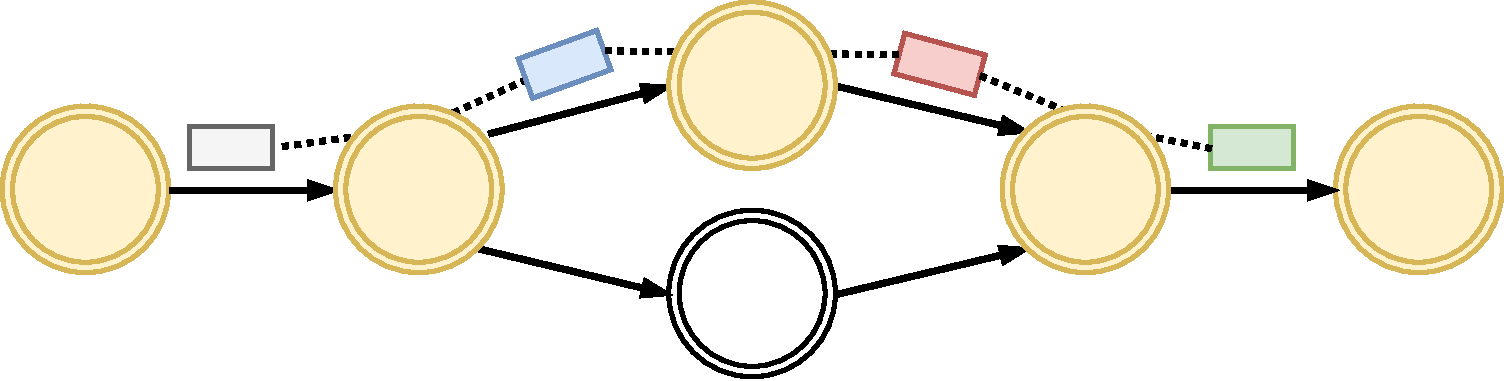
\includegraphics[width=0.9\linewidth]{pics/logical-graph}
    \caption{A logical execution  graph}
    \label{logical-graph-figure}
  \end{minipage}%
  \begin{minipage}[b]{.5\textwidth}
    \centering
    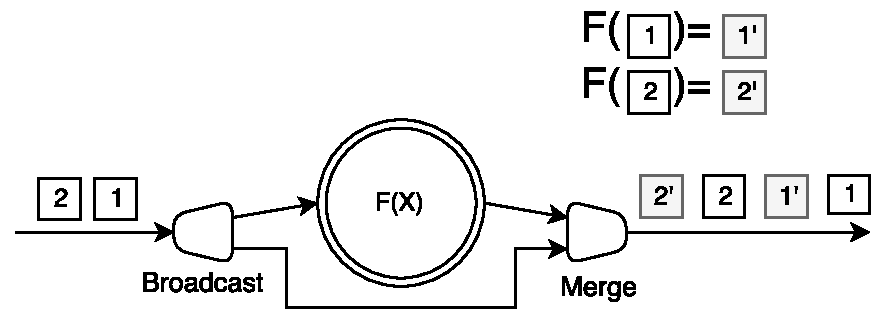
\includegraphics[width=\linewidth]{pics/ordering}
    \caption{The ordering model}
    \label{ordering}
  \end{minipage}
\end{figure}

Data items are totally ordered according to labeles assigned to events at the entry as a part of meta-information. All operations preserve this order. Any additional items produced by an operation are placed between the item being processed and the next item. The ordering labels are dropped when items are delivered from the barrier. 

The ordering is illustrated  in Figure~\ref{ordering}. Data item with payload $1'$ is the derivative of the item with payload $1$, according to operation $F$. The same is for items with payloads $2'$ and $2$. After merge operation, the order between $1$ and $2$ is preserved. Furthermore, $1'$ follows $1$, and $2'$ follows $2$.  


The list of available operations includes:
\begin {description}
  \item [Map] applies a user-defined function to the payload of an input item and returns a (possibly empty) sequence of data items with transformed payloads. 

  \item [Broadcast] replicates an input item to the specified number of operations.

  \item [Merge] operation is initialized with the specified number of input nodes. It sends all incoming data to the output.

  \item [Grouping] constructs a single item containing a set of consecutive items that have the same value of partition function. The maximum number of items that can be grouped is specified as a parameter  $Window Size$. 
    
  The output item of the grouping has the same ordering label as the last item in the output group. Groupings of different partitions are independent. Grouping is the only operation that has a state.
\end {description}

The following example illustrates  the grouping operation. Let the input stream be a series of integers: $ 1,2,3, \ldots$, and the  partition function returns for even numbers and 0 otherwise. If the window is set to 3, the output is 
$$(1), (2), (1|3), (2|4), (1|3|5), (2|4|6), (3|5|7), (4|6|8), \ldots$$
